\documentclass[conference]{IEEEtran}
\IEEEoverridecommandlockouts
% The preceding line is only needed to identify funding in the first footnote. If that is unneeded, please comment it out.
\usepackage{cite}
\usepackage[ngerman]{babel}
\usepackage[utf8]{inputenc}
\usepackage{amsmath,amssymb,amsfonts}
\usepackage{algorithmic}
\usepackage{graphicx}
\usepackage{textcomp}
\usepackage{xcolor}
\usepackage{listings}


\definecolor{pblue}{rgb}{0.13,0.13,1}
\definecolor{pgreen}{rgb}{0,0.5,0}
\definecolor{pred}{rgb}{0.9,0,0}
\definecolor{pgrey}{rgb}{0.46,0.45,0.48}
\lstset{language=Python,
	showspaces=false,
	showtabs=false,
	breaklines=true,
	tabsize=2,
	showstringspaces=false,
	breakatwhitespace=true,
	commentstyle=\color{pgreen},
	keywordstyle=\color{pblue},
	stringstyle=\color{pred},
	basicstyle=\ttfamily
}


\usepackage{url}
\def\BibTeX{{\rm B\kern-.05em{\sc i\kern-.025em b}\kern-.08em
		T\kern-.1667em\lower.7ex\hbox{E}\kern-.125emX}}
\begin{document}
	
	\title{Videoanalyse und Objekttracking}
	
	\author{\IEEEauthorblockN{1\textsuperscript{st} Bartolovic Eduard}
	\IEEEauthorblockA{\textit{Hochschule München} \\
		München, Deutschland \\
		eduard.bartolovic0@hm.edu}
	\and
	\IEEEauthorblockN{2\textsuperscript{nd} Thomas Willeit}
	\IEEEauthorblockA{\textit{Hochschule München} \\
		München, Deutschland \\
		XXXXX@hm.edu}
	\and
	\IEEEauthorblockN{3\textsuperscript{rd} Schäfer Julia}
	\IEEEauthorblockA{\textit{Hochschule München} \\
		München, Deutschland \\
		j.schaefer0@hm.edu}
	}

	
	\maketitle
	
	\begin{abstract}
		
	\end{abstract}
	
	\section{Konzept}
	Ziel des Projektes ist es klassische Verfahren mit neuere DeepLearning Verfahren zu vergleichen.
	Dafür ist für beide arten eine Pipeline geschaffen worden.\\
	Für die Klassische Verfahren wurde für die Objekterkennung Gausmixture verwendet und für das Tracking Sort. Für die DeepLearnig Verfahren wurde für die Objekterkennung ein Neuronales Netz  und für das Tracking wurde Deepsort verwendet.
	
	\begin{figure}[h]
		\begin{center}
			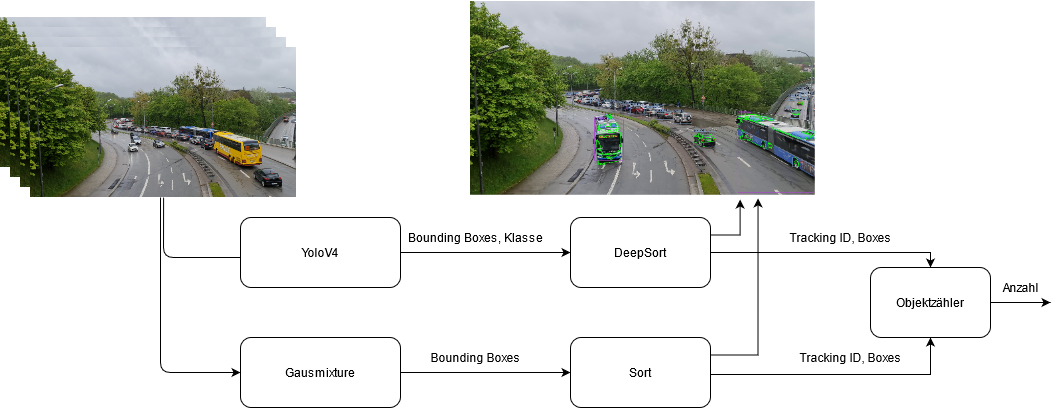
\includegraphics[width=14cm]{Media/KonzeptVAOT.png}
			\caption{Konzept für das Projekt}
			\label{Konzept}
		\end{center}
	\end{figure}
	
	\section{Objekterkennung: Gauß Mixture}
	
	\section{Objekterkennung: YoloV4}
	YOLO ist ein Neuronal Netz für die Echtzeit-Objekterkennung. YOLO ist die Abkürzung für 'You Only Look Once' was übersetzt 'Man sieht nur einmal hin' heißt. Es zerlegt die Aufgabe der Objekterkennung in zwei Teile. Einmal in die Objektposition über Bounding Boxes und dann in Klassifizierung zur Bestimmung der Objektklasse.\\
	Dieses System basiert auf Residualblöcken, Bounding-Box-Regression und IOU-Techniken.
	Das Bild in ein S × S-Gitter mit den Residualblöcken aufgeteilt. Wenn der Mittelpunkt eines Objekts in eine Gitterzelle fällt, ist diese Gitterzelle für die Erkennung dieses Objekts zuständig. Jede Gitterzelle sagt B Bounding Boxes und Konfidenzwerte für diese Boxen voraus \cite{b1}.......\\
	In diesem Projekt verwendeten wir die 4te und damit aktuell neueste Version von Yolo\cite{b2}. So bietet jede Version inkrementelle Verbesserung zum jeweiligen Vorgänger.\\
	Unser Modell wurde bereits mit dem Microsoft COCO Datensatz trainiert worden. Es sind 80 verschiedene Klassen erkennbar. Wir interessieren uns aber nur für einen kleineren Teil wie:
	\begin{enumerate}
		\item Personen
		\item Pkw
		\item Lkw
		\item Busse
		\item Fahrräder
		\item Züge
	\end{enumerate}
	Je nach Szenario lassen sich per Parameter die relevanten Klassen auswählen. Das Modell prädiktiert trotzdem noch alle Klassen. Die nicht relevanten werden einfach im Postprocessing herausgefiltert. Das Ergebnis einer Prädiktion ist eine Liste von Objekten welches aus den x,y Koordinate der oberen linken Punktes der Boundingbox, der Breite w, der Höhe h, der Klasse und des Konfidenzwerts. 
	
	\subsection{Fehler in der Erkennung}
	...falsch Klassifizierung wegen schlechter Datensatz....
	Zu großer Datensatz...

	\section{Tracking: Sort}
	
	\section{Tracking: DeepSort}
	
	\section{Zählen von Objekten}
	
	\section{Zustandserkennung Züge}
	
	\begin{thebibliography}{00}
		\bibitem{b1}https://arxiv.org/pdf/1506.02640.pdf
		\bibitem{b2}https://arxiv.org/pdf/2004.10934.pdf
	\end{thebibliography}
	
	
	
	\section{Anhang}
	

\end{document}
